\chapter{Results}

\section{Pairwise $T^p$ - $T^-$}
From the initial runs where two parameters were changed at a time, the following were observed:
\begin{enumerate}
  \item Only when $T^p$ is not severely testosterone limited ($ul_{test,T^p}$ is low), $T^p$ can coexist with or outcompete $T^-$ as shown in \autoref{fig_Tpro-Tneg_testlims}. In every other case, $T^-$ drives $T^p$ to extinction.
  \item These competitive outcomes are also dependent on the initial proportion of $T^p$, all the other parameters being the same as shown in  \autoref{fig_Tpro-Tneg_testlims}.
  \item  When $T^-$ is strongly oxygen-limited ($ll_{O_2,T^-} \geq 0.6$) but $T^p$ is also limited by testosterone. In this case, $T^-$ wins out eventually as oxygen levels rise faster than testosterone through the external supply term, $p_{O_2}$ as shown in \autoref{fig_Tpro-Tneg_o2lims}.
  \item When $T^-$ is oxygen limited but with poor oxygen production (lower $p_{O_2}$), $T^p$ is able to drive $T^-$ to extinction as $T^p$ can grow and consume enough oxygen to keep the oxygen levels below those required for $T^-$ to grow as shown in \autoref{fig_Tpro-Tneg_o2lims}.
\end{enumerate}

\begin{figure}[h!]
  \centering
  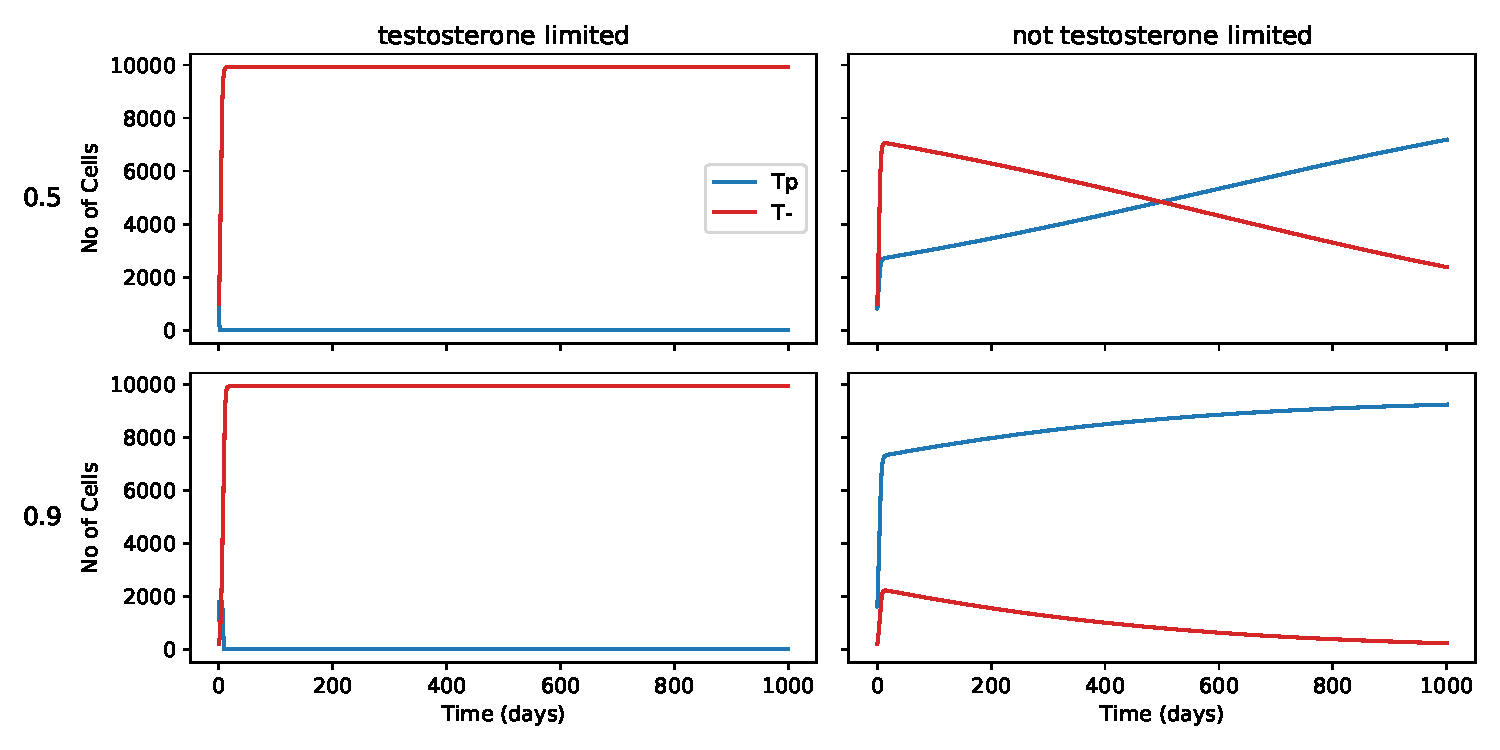
\includegraphics[width=\textwidth]{Tpro-Tneg_testlims}
  \caption[Pairwise $T^p - T^-$ timeseries, testosterone limitation]{Pairwise $T^p - T^-$ timeseries, when $T^p$ is testosterone limited and not testosterone limited (columns) and at different initial proportions of $T^p$ (rows). $T^p$ is testosterone limited at $ul_{test,T^p}=0.5$ and not testosterone limited at $ul_{test,T^p}=0.1$.}
  \label{fig_Tpro-Tneg_testlims}
\end{figure}

\begin{figure}[h!]
  \centering
  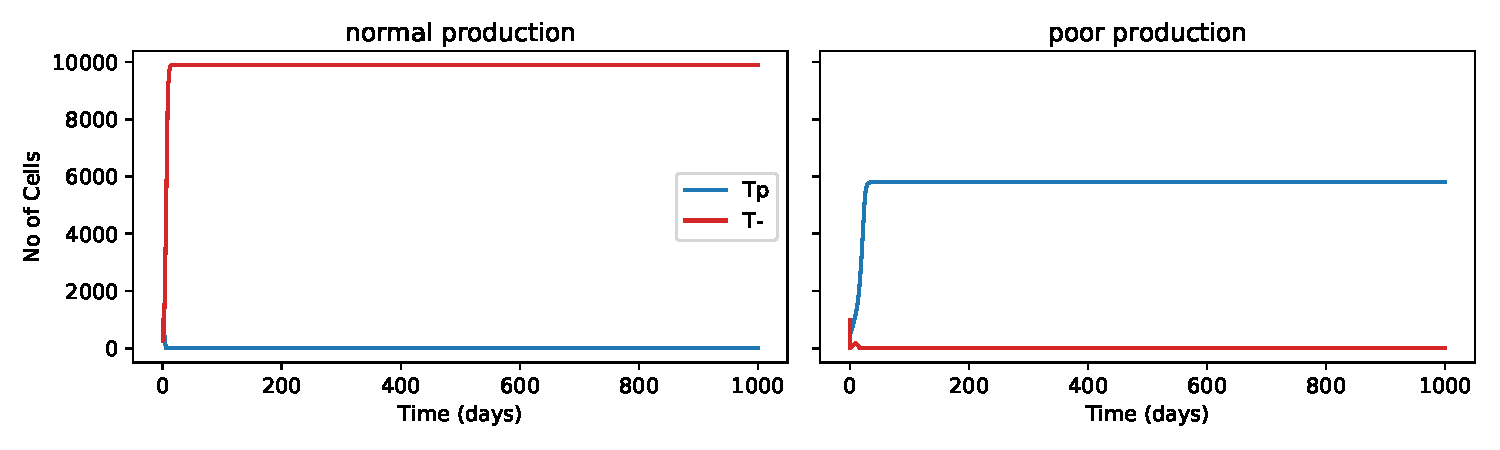
\includegraphics[width=\textwidth]{Tpro-Tneg_o2lims}
  \caption[Pairwise $T^p - T^-$ timeseries, oxygen limitation]{Pairwise $T^p - T^-$ timeseries, when $T^-$ is oxygen limited and at different oxygen production (column). $T^-$ is oxygen limited at $ll_{O_2,T^-}=0.6$ and $T^p$ is testosterone limited at $ul_{test,T^p}=0.5$. The normal and poor production of oxygen are 0.11 and 0.0675 min$^{-1}$ respectively}
  \label{fig_Tpro-Tneg_o2lims}
\end{figure}

Additionally, a brute force parameter space exploration was done over a large combination of parameters. Due to the large parameter set, interpreting the results is difficult and only a few generalised observations were found, as listed below.
\begin{enumerate}
  \item $T^-$ drives $T^p$ to extinction when $ll_{O_2,T^p} \geq 0.6$, regardless of the other parameters, in other words, $T^p$ shouldn't be limited by oxygen to compete with $T^-$.
  \item $T^-$ drives $T^p$ to extinction when $ll_{test,T^p} \geq 0.2$, regardless of the other parameters, in other words, $T^p$ needs to be able to grow even on the smallest amount of testosterone to compete with $T^-$.
  \item $T^-$ drives $T^p$ to extinction when $ul_{test,T^p} \geq 0.3$ and $ll_{O_2,T^-} \leq 0.4$ but not when $ll_{O_2,T^-} \geq 0.6$, in other words, $T^p$ shouldn't be testosterone limited when $T^-$ is not oxygen limited to be to compete with $T^-$. The $ul_{test,T^p}$ required for $T^p$ to not go extinct also increases with increased $ll_{O_2,T^-}$, that is, $T^p$ can afford to be more testosterone limited as $T^-$ becomes more oxygen limited.
\end{enumerate}

From the above observations, the following cases were formulated as an exhaustive formulation of possible conditions. Three levels of $T^p\ test$ limitation: no, moderate and severe corresponding to $ul_{test,T^p}=0.1, 0.3, 1$ respectively, $T^-\ O_2$ limitation: no, high and severe corresponding to $ll_{O_2,T^-}=0, 0.6, 0.8$ respectively, and $O_2$ production: normal and poor corresponding to $p_{O_2}=0.11, 0.0675$ min$^{-1}$ respectively were considered and pairwise competitive runs were done over all combinations of these with varying initial cell seeding.
\begin{longtable}[c]{|l|l|l|}

  \hline \multicolumn{1}{|c|}{\textbf{$O_2$ production}} & \multicolumn{1}{c|}{\textbf{$T^-\ O_2$ limitation}} & \multicolumn{1}{c|}{\textbf{$T^p\ test$ limitation}}\\ \hline
  \endhead

  \hline \multicolumn{3}{|r|}{{Continued on next page}} \\ \hline
  \endfoot

  \endlastfoot

  normal & no & no \\ \hline
  normal & no & moderate \\ \hline
  normal & no & severe \\ \hline
  normal & high & no \\ \hline
  normal & high & moderate \\ \hline
  normal & high & severe \\ \hline
  normal & severe & no \\ \hline
  normal & severe & moderate \\ \hline
  normal & severe & severe \\ \hline
  poor & no & no \\ \hline
  poor & no & moderate \\ \hline
  poor & no & severe \\ \hline
  poor & high & no \\ \hline
  poor & high & moderate \\ \hline
  poor & high & severe \\ \hline
  poor & severe & no \\ \hline
  poor & severe & moderate \\ \hline
  poor & severe & severe \\ \hline

  \caption{Table of cases for $T^p$ - $T^-$ pairwise}
  \label{tab_Tpro-Tneg_cases}
\end{longtable}

\begin{figure}[h!]
  \centering
  \begin{subfigure}[b]{\textwidth}
    \centering
    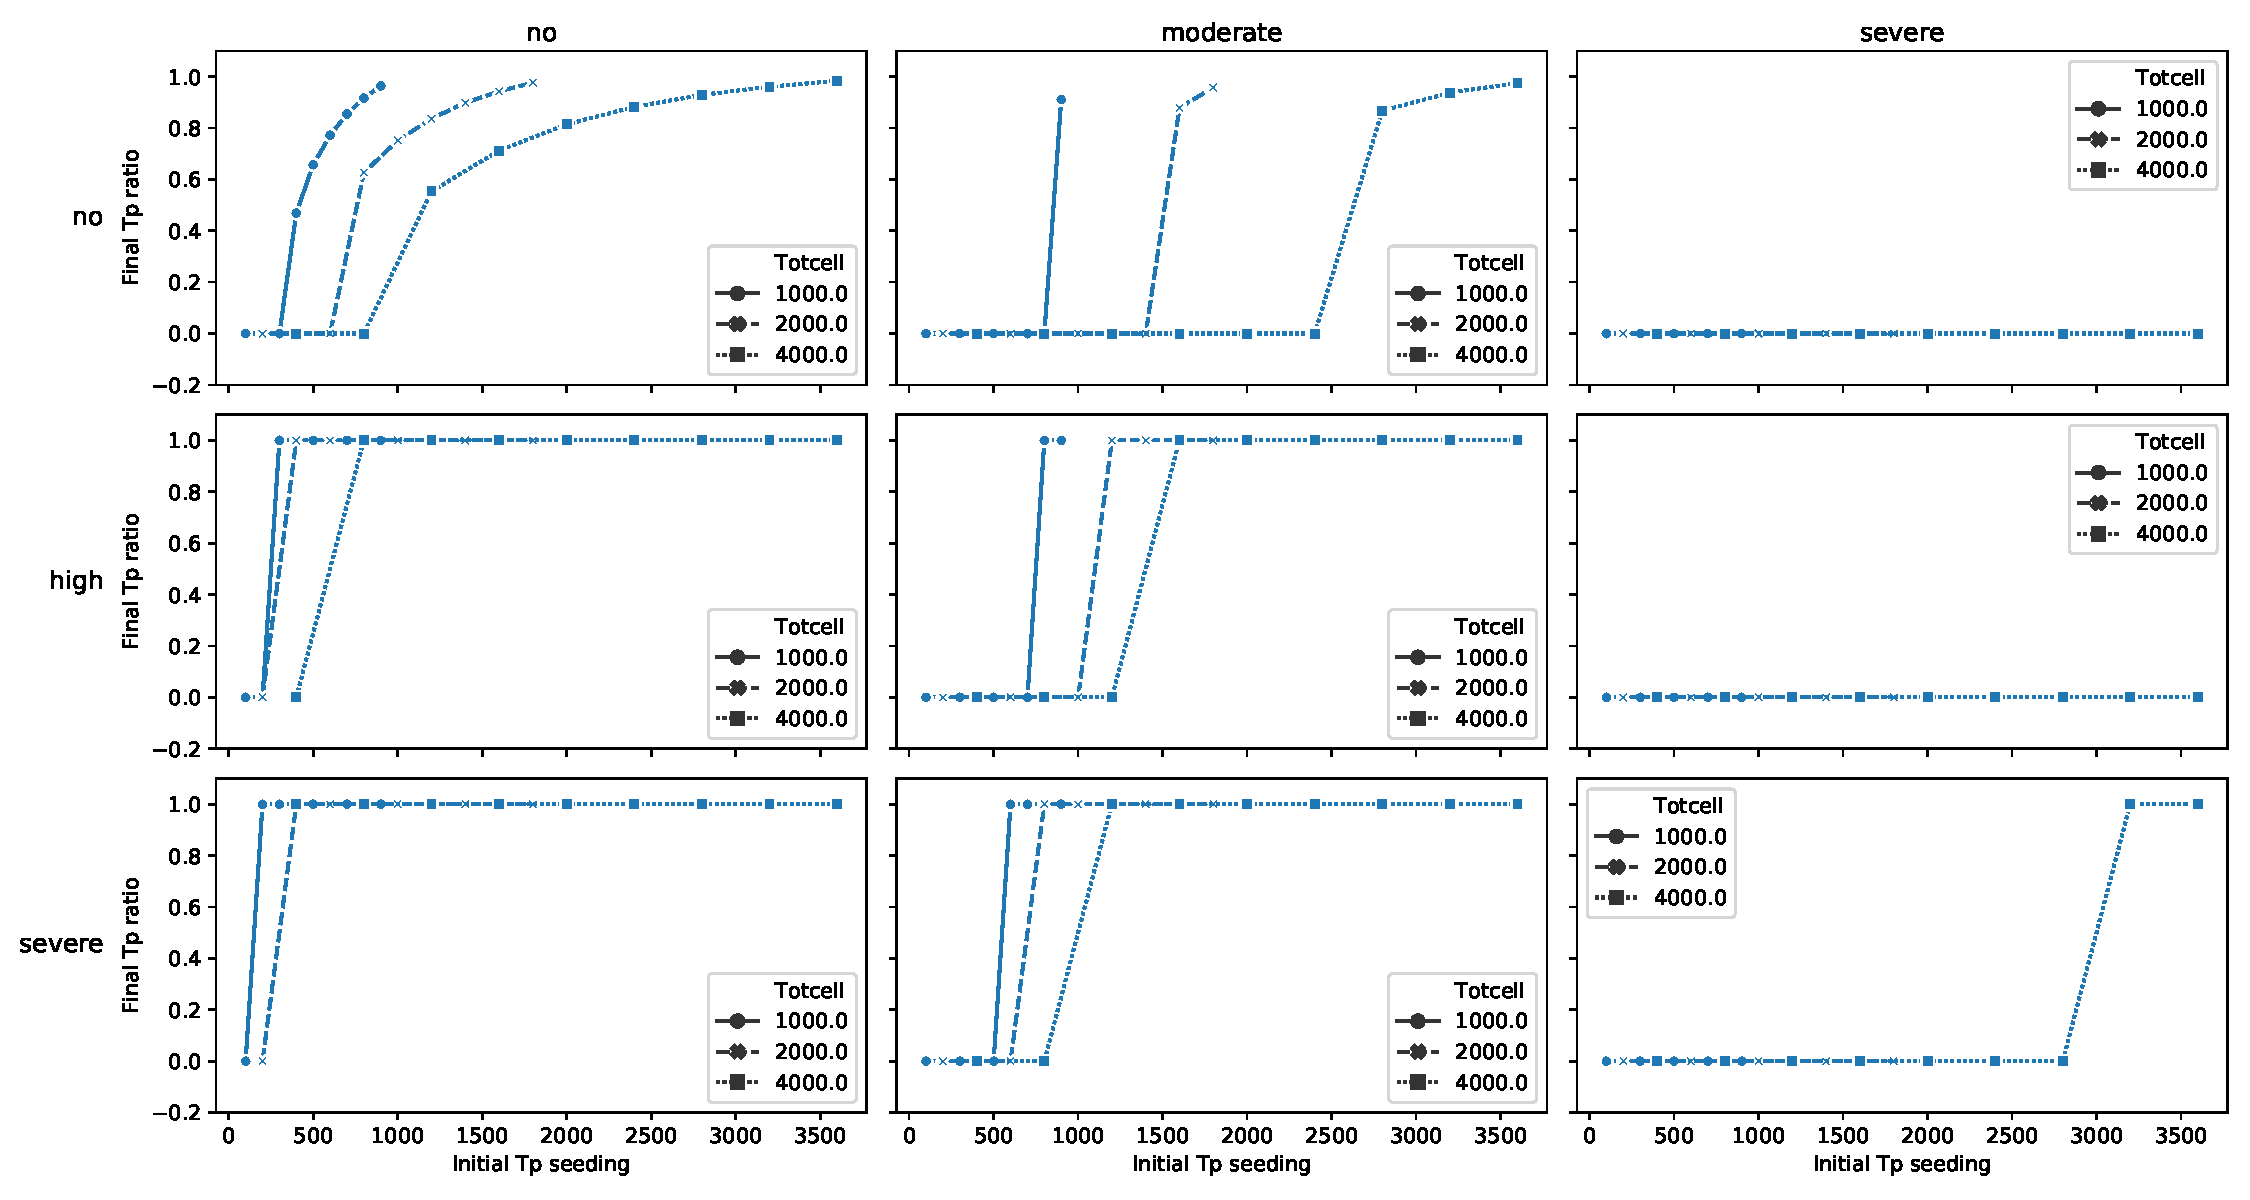
\includegraphics[width=\textwidth]{Tpro-Tneg_cases_normal}
    \caption{normal production}
    \label{fig_Tpro-Tneg_cases_normal}
  \end{subfigure}
  \begin{subfigure}[b]{\textwidth}
    \centering
    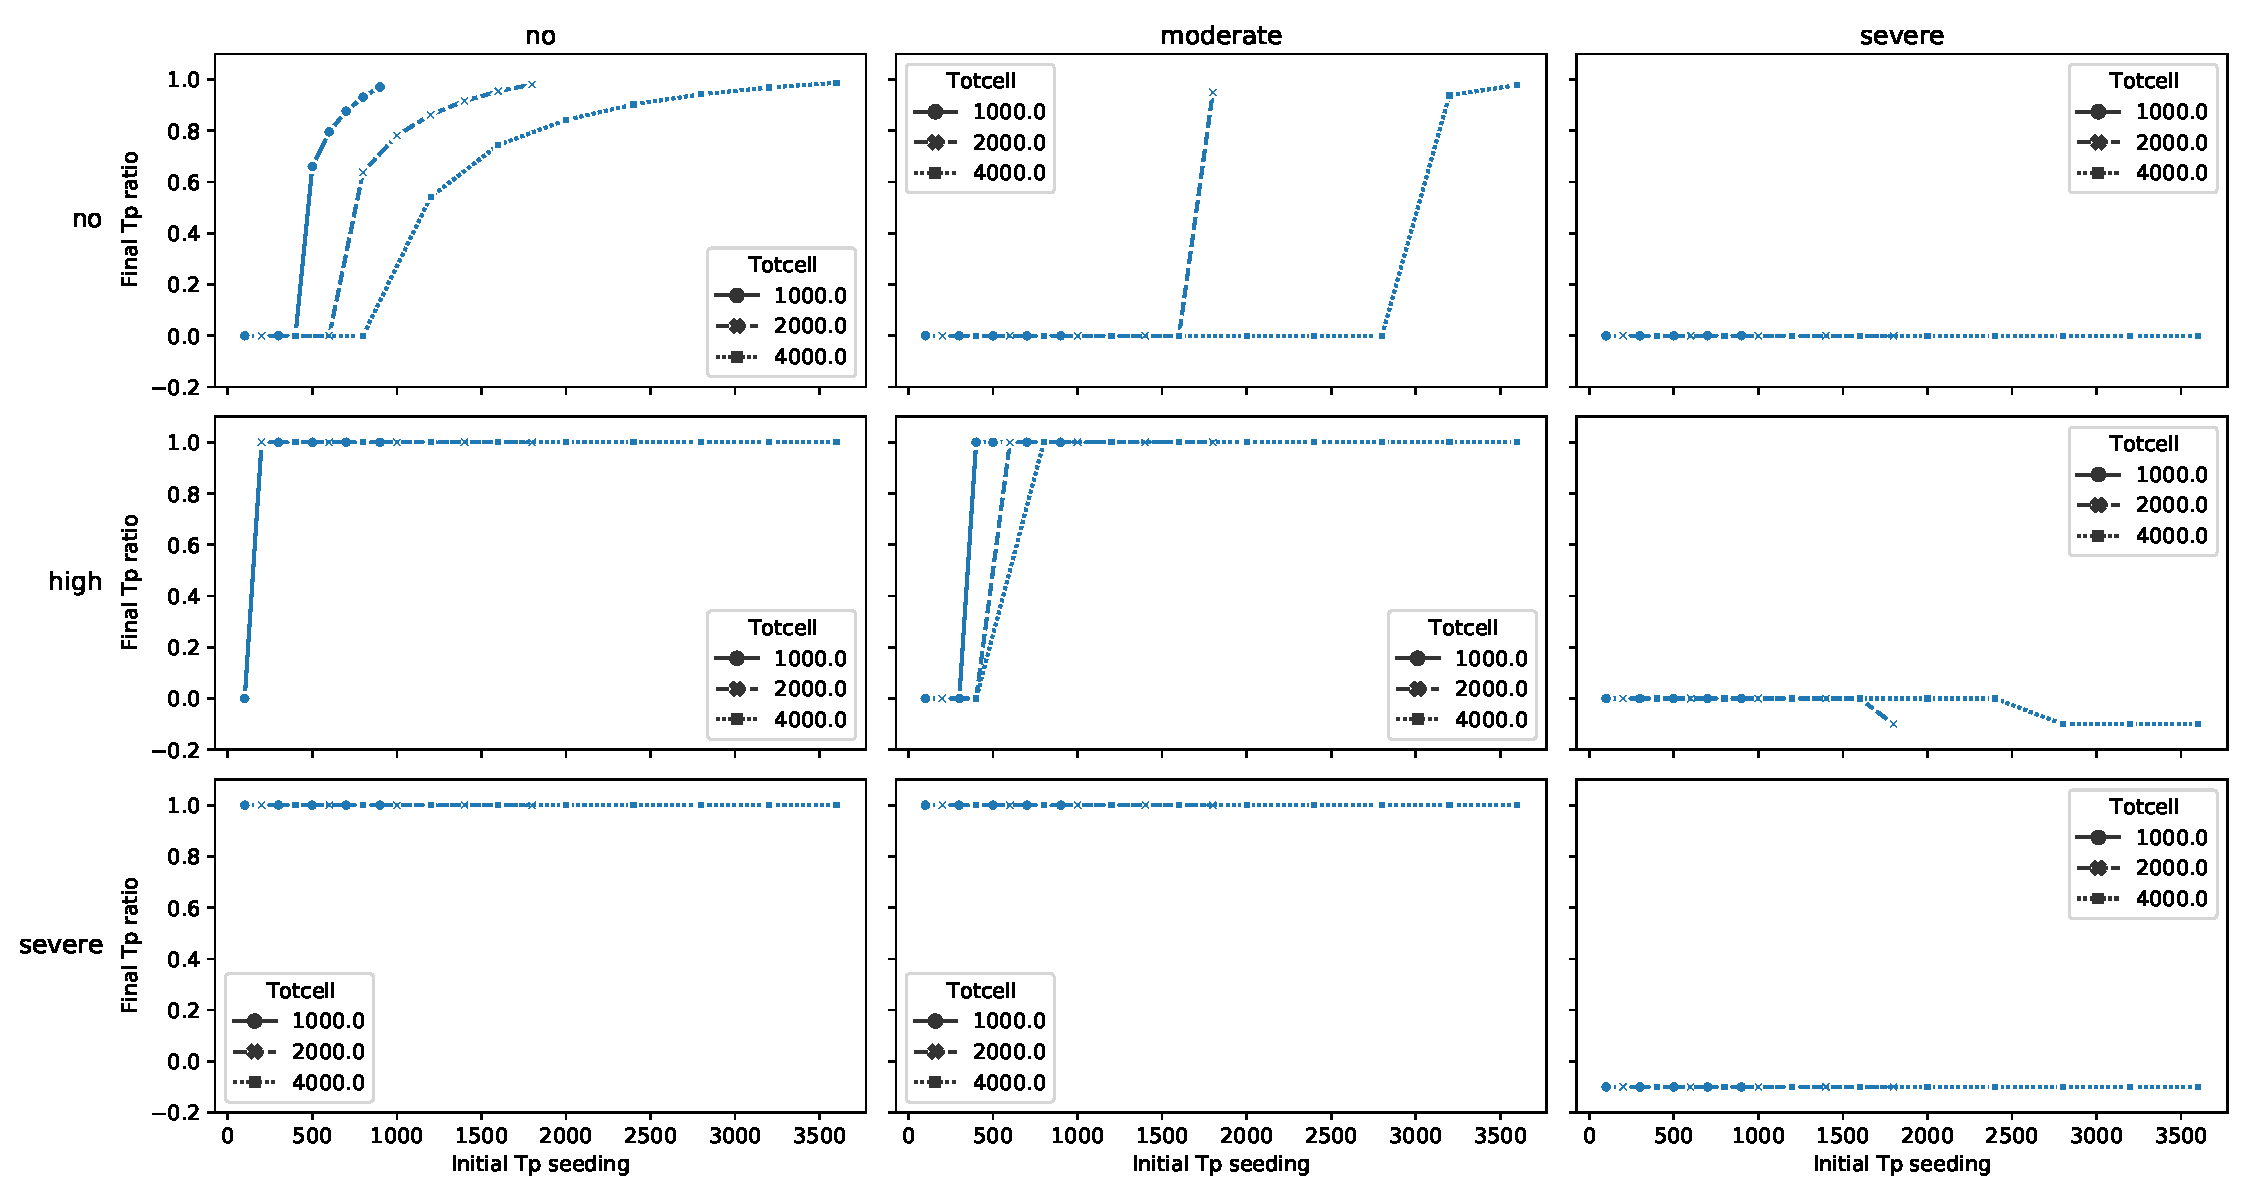
\includegraphics[width=\textwidth]{Tpro-Tneg_cases_poor}
    \caption{poor production}
    \label{fig_Tpro-Tneg_cases_poor}
  \end{subfigure}
  \caption[Final $T^p$ ratio of pairwise $T^p - T^-$ runs under different cases]{Final $T^p$ ratio of pairwise $T^p - T^-$ runs under different cases. Subfigures: $O_2$ Production, Rows: $T^-\ O_2$ limitation, Columns: $T^p\ test$ limitation. Note: Ratio = -0.1 is used when both cell types go extinct.}
  \label{fig_Tpro-Tneg_cases}
\end{figure}

\newpage
The following were observed from the cases as visualised in \autoref{fig_Tpro-Tneg_cases}:
\begin{enumerate}
  \item Coexistence is observed only when there is low or moderate limitation of testosterone for $T^p$ and have no limitation of oxygen for $T^-$. For low $T^p$ initial seeding, $T^-$ dominates over $T^p$ and causes it to go extinct, but as $T^p$ initial seeding increases the favour shift towards $T^p$.
  \item $T^-$ causes $T^p$ to go extinct for all initial seedings when $T^p$ is severely testosterone limited. Even with a high initial seeding advantage, $T^-$ grows, overtakes $T^p$ and eventually causes $T^p$ to go extinct. $T^-$ also goes exitinct in this case if it is limited by oxygen under poor oxygen production. Despite this $T^p$ is weighed down by both the testosterone limitation and density-dependent competition of the remaining $T^-$ cells and goes extinct as a result.
  \item The outcome switches from $T^p$ going extinct to $T^-$ going extinct for higher $T^p$ initial seeding when $T^-$ is highly limited by oxygen under either poor or normal oxygen production and when $T^-$ is severely limited by oxygen under normal oxygen production. Similar to the cases with co-existence, for low $T^p$ initial seeding, $T^-$ dominates over $T^p$ and causes it to go extinct, but as $T^p$ initial seeding increases the favour shift towards $T^p$. However, in this case the oxygen levels don't go above the levels required for $T^-$ to grow before it goes extinct and only $T^p$ remains.
  \item $T^-$ goes extinct for all initial seedings when it is severely oxygen limitied under poor oxygen production. The oxygen limitation on $T^-$ is too high and the oxygen levels never reach the levels required for a non-zero growth for $T^-$.
  \item Additionally, total population size has weaker effect than initial proportion for the dynamics and outcomes for each particular case.
\end{enumerate}

\section{Pairwise $T^+$ - $T^p$}
From the initial runs where two parameters were changed at a time, the following were observed:
\begin{enumerate}
    \item When $T^p$ limited by testosterone more than $T^+$ ($ul_{test,Tp} > ul_{test,T+}$), $T^+$ can consume and grow on the limited testosterone present, and this is enough for the density-dependent competition to drive $T^p$ to extinction. Without $T^p$ to provide testosterone, $T^+$ subsequently goes extinct.
    \item When $T^p$ is weakly limited by testosterone relative to $T^+$ ($ul_{test,Tp} \leq ul_{test,T+}$), both cells coexist. Due to weaker testosterone limitation, $T^p$ can grow faster initially and secrete enough testosterone for $T^+$ without being negatively affected by $T^+$. This is visualised in \autoref{fig_Tpos-Tpro_testlims}.
    \item In the above case, the proportion of $T^+$ in the final population decreases as $T^+$ becomes more testosterone limited.
    \item When both are severely testosterone limited but not oxygen limited, $T^p$ causes $T^+$ to go extinct. However, in a special scenario when both are oxygen limited with $T^+$ being more limited, coexistence is observed. A balance of sort is achieved here, where, in the initial period of low oxygen, $T^p$ can grow more than $T^+$ and secrete enough testosterone to sustain both population but doesn't grow as much as to drive $T^+$ to extinction. This is visualised in \autoref{fig_Tpos-Tpro_o2lims}.
  \end{enumerate}

\begin{figure}[h!]
  \centering
  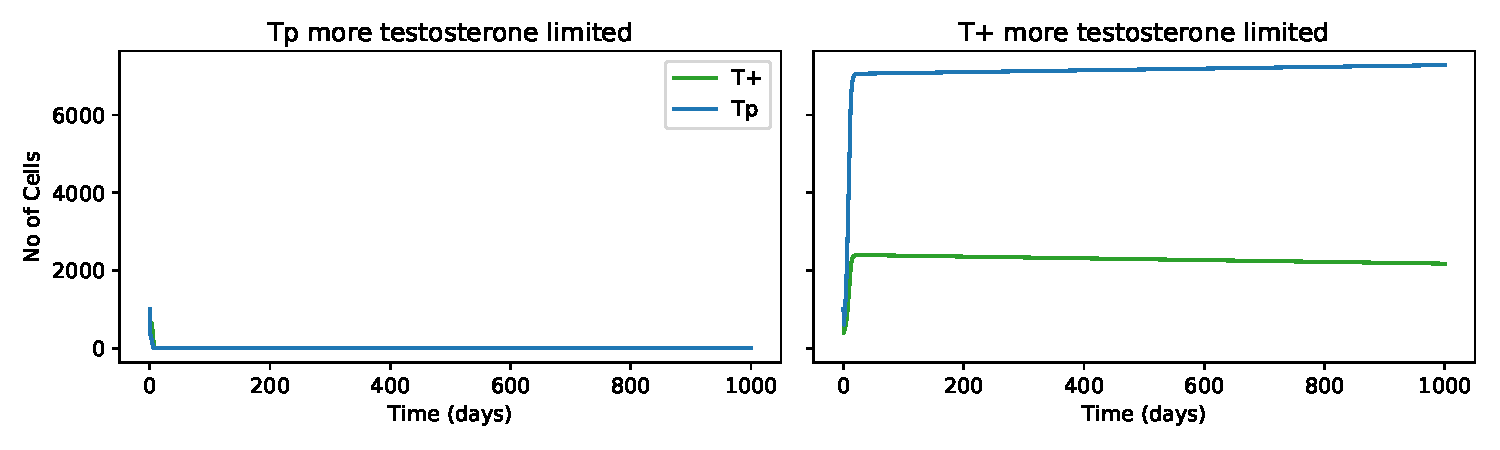
\includegraphics[width=\textwidth]{Tpos-Tpro_testlims}
  \caption[Pairwise $T^+ - T^p$ timeseries, testosterone limitation]{Pairwise $T^+ - T^p$ timeseries, when $T^p$ is more testosterone limited than $T^p$ and when $T^+$ is more testosterone limited than $T^p$. $T^p$ is more limited testosterone limited at $ul_{test,T^+}=0.3,ul_{test,T^p}=0.5$ and $T^+$ is limited more at $ul_{test,T^+}=0.5,ul_{test,T^p}=0.3$.}
  \label{fig_Tpos-Tpro_testlims}
\end{figure}

\begin{figure}[h!]
  \centering
  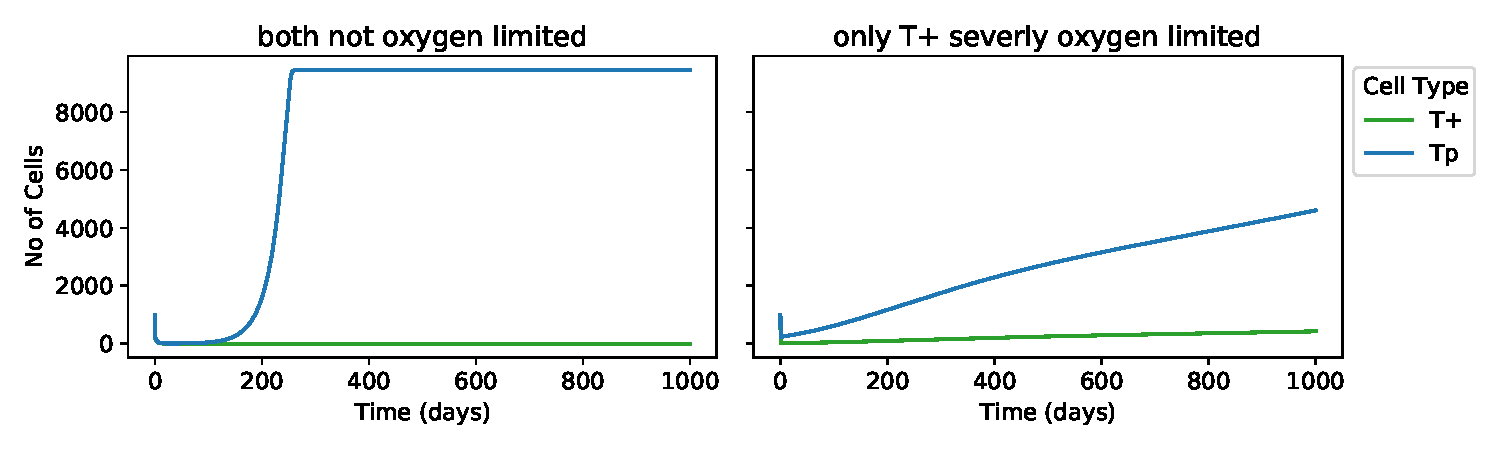
\includegraphics[width=\textwidth]{Tpos-Tpro_o2lims}
  \caption[Pairwise $T^+ - T^p$ timeseries, oxygen limitation]{Pairwise $T^+ - T^p$ timeseries, when both cell types are testosterone limited and not oxygen limited at $ll_{O_2,T^+}=0.0, ll_{O_2,T^p}=0.0$ and $T^+$ is oxygen limited and $T^p$ moderately at $ll_{O_2,T^+}=0.6, ll_{O_2,T^p}=0.4$.}
  \label{fig_Tpos-Tpro_o2lims}
\end{figure}

\newpage

From the above observations, the following cases were formulated as an exhaustive formulation of possible conditions. Three levels each of $T^p\ test$ and $T^+\ test$ limitation: no, moderate and severe corresponding to $ul_{test,T^i}=0.1, 0.3, 1$ respectively, Three levels each of $T^p\ O_2$ and $T^+\ O_2$ limitation: no, moderate and severe corresponding to $ll_{O_2,T^i}=0, 0.4, 0.8$  respectively were considered and pairwise competitive runs were done over some combinations of these with varying initial cell seeding.\\
Only two levels of limitiations were considered for each resource when combinations of both $O_2$ or $test$ limitations were done to reduce the number of combinations for better interpretability. Similarly, different levels of $O_2$ or $test$ production is not considered in these cases for the same reason. Production terms will ultimately affect resource availability, and we're doing something roughly similar by adjusting the response function of the cell instead of actual resource concentrations.

\begin{longtable}[c]{|l|l|l|l|}

  \hline  \multicolumn{1}{|c|}{\textbf{$T^+\ O_2$ limitation}} & \multicolumn{1}{c|}{\textbf{$T^p\ O_2$ limitation}} & \multicolumn{1}{c|}{\textbf{$T^+\ test$ limitation}} & \multicolumn{1}{c|}{\textbf{$T^p\ test$ limitation}}  \\ \hline
  \endhead

  \hline \multicolumn{4}{|r|}{{Continued on next page}} \\ \hline
  \endfoot

  \endlastfoot
  no & no & no & no \\ \hline
  no & no & no & moderate \\ \hline
  no & no & no & severe \\ \hline
  no & no & moderate & no \\ \hline
  no & no & moderate & moderate \\ \hline
  no & no & moderate & severe \\ \hline
  no & no & severe & no \\ \hline
  no & no & severe & moderate \\ \hline
  no & no & severe & severe \\ \hline
  no & moderate & no & no \\ \hline
  no & moderate & no & moderate \\ \hline
  no & moderate & moderate & no \\ \hline
  no & moderate & moderate & moderate \\ \hline
  no & severe & no & no \\ \hline
  moderate & no & no & no \\ \hline
  moderate & no & no & moderate \\ \hline
  moderate & no & moderate & no \\ \hline
  moderate & no & moderate & moderate \\ \hline
  moderate & moderate & no & no \\ \hline
  moderate & moderate & no & moderate \\ \hline
  moderate & moderate & moderate & no \\ \hline
  moderate & moderate & moderate & moderate \\ \hline
  moderate & severe & no & no \\ \hline
  severe & no & no & no \\ \hline
  severe & moderate & no & no \\ \hline
  severe & severe & no & no \\ \hline
  \caption{Table of cases for $T^+$ - $T^p$ pairwise}
  \label{tab_Tpro-Tneg_cases}

\end{longtable}

The following were observed from the different cases. For better visualization, the figures are divided into testosterone limitations in \autoref{fig_Tpos-Tpro_cases_test}, oxygen limitations in \autoref{fig_Tpos-Tpro_cases_o2} and combinations of the limitations in \autoref{fig_Tpos-Tpro_cases_combi}.
\begin{enumerate}
  \item Severe limitation of either oxygen or testosterone for $T^+$ relative to $T^p$ causes it to go extinct. In a special case, when $T^p$ numbers are high enough to produce an excess of testosterone, a small fraction of $T^+$ survives regardless of the strength of $T^+$ test limitation. Conversely, when neither resource is limiting, co-existence occurs at all seeding densities and proportions of $T^p$, which suggests that competitive exclusion of either cell type is strongly dependent on environmental conditions and resource limitation. When $T^+$ is moderately oxygen limitied relative to $T^p$, $T^+$ can coexist at low initial density of $T^p$ but goes extinct at higher initial densities.
  \item Similarly, $T^p$ is driven to extinction in every case where $T^p$ limitation of either oxygen or testosterone is severe relative to $T^+$ limitation of the same resource. Extinction of $T^p$ then leads to extinction of $T^+$ trivially. Such is the case for the most part with moderate limitation of testosterone for $T^p$ relative to $T^+$. However, this $T^p$ extinction is seen to rescued for higher initial density of $T^p$ relative to $T^+$ as this allows the former to overcome competition, leading to co-existence.
  \item However, with moderate limitation of oxygen for $T^p$ relative to $T^+$. $T^+$ despite having a growth advantage due to the lowered oxygen limitation compared to $T^p$, still requires testosterone $T^p$ for survival and reduces its growth and inhibition on $T^p$ to allow it to secrete enough testosterone. Interestingly, this is also the case with co-existence at lower final $T^p$ proportions than any other case.
  \item In very broad terms, co-existence is more common when the strength of limitation of either resource is the same for both cell types-these are the main diagonals in \autoref{fig_Tpos-Tpro_cases_test} and \autoref{fig_Tpos-Tpro_cases_o2}. However, under severe limitation of testosterone for both cell types, increasing relative proportion gives a competitive edge to $T^p$ presumably by increasing net availability of testosterone in the system. This increased availability also has limits beyond which further increase in $T^p$ proportion is marginally detrimental to $T^p$ success.
  \item Similarly, co-existence is observed when $T^+$ is moderately testosterone limitied relative to $T^p$. However, in this case, lower initial proportion of $T^p$ favours $T^p$ and leads to a dip in the plot. At low initial proportion of $T^p$, $T^+$ being limited by testosterone dies out until sufficient testosterone is established and this might give and advantage for $T^p$ to establish a larger population before $T^+$ has the capacity to compete.
  \item The behaviour of the system when both the cells are moderately limited either by testosterone or oxygen is very similar to the cases when both the cells were not limited by either testosterone or oxygen. Although, with the higher testosterone limitations of $T^p$, a higher $T^p$ initial seeding is required to have $T^p$ overcome suppression by $T^+$. Additionally, when $T^p$ is moderately limited by oxygen relative to $T^+$, the higher testosterone limitation of $T^+$ leads to higher $T^p$ required for testosterone and a higher final $T^p$ population compared to the case without any testosterone limitations.
  \item When both testosterone and oxygen are moderately limiting for a cell type relative to the other, the combined overall limitation is severe and that particular cell type is driven to extinction similar to when only one resource was severely limiting.
  \item When $T^p$ is moderately limited by oxygen relative to $T^+$ and $T^+$ moderately limited by testosterone relative to $T^p$, a balance is achieved. $T^+$ can outcompete $T^p$ due to the excess oxygen but soon is limited by testosterone and has to allow a sizeable population of $T^p$ to grow to maintain the required testosterone levels. However, with the inverse case where $T^p$ is testosterone limited and $T^+$ is oxygen limited, the outcomes are unstable and it switches from $T^p$ going extinct and $T^+$ in extension at low initial proportion to $T^+$ going extinct for higher initial proportion.
  \item Additionally, total population size has weaker effect than initial proportion for the dynamics and outcomes for each particular case.
\end{enumerate}

\begin{figure}[h!]
  \centering
  \begin{subfigure}[b]{\textwidth}
    \centering
    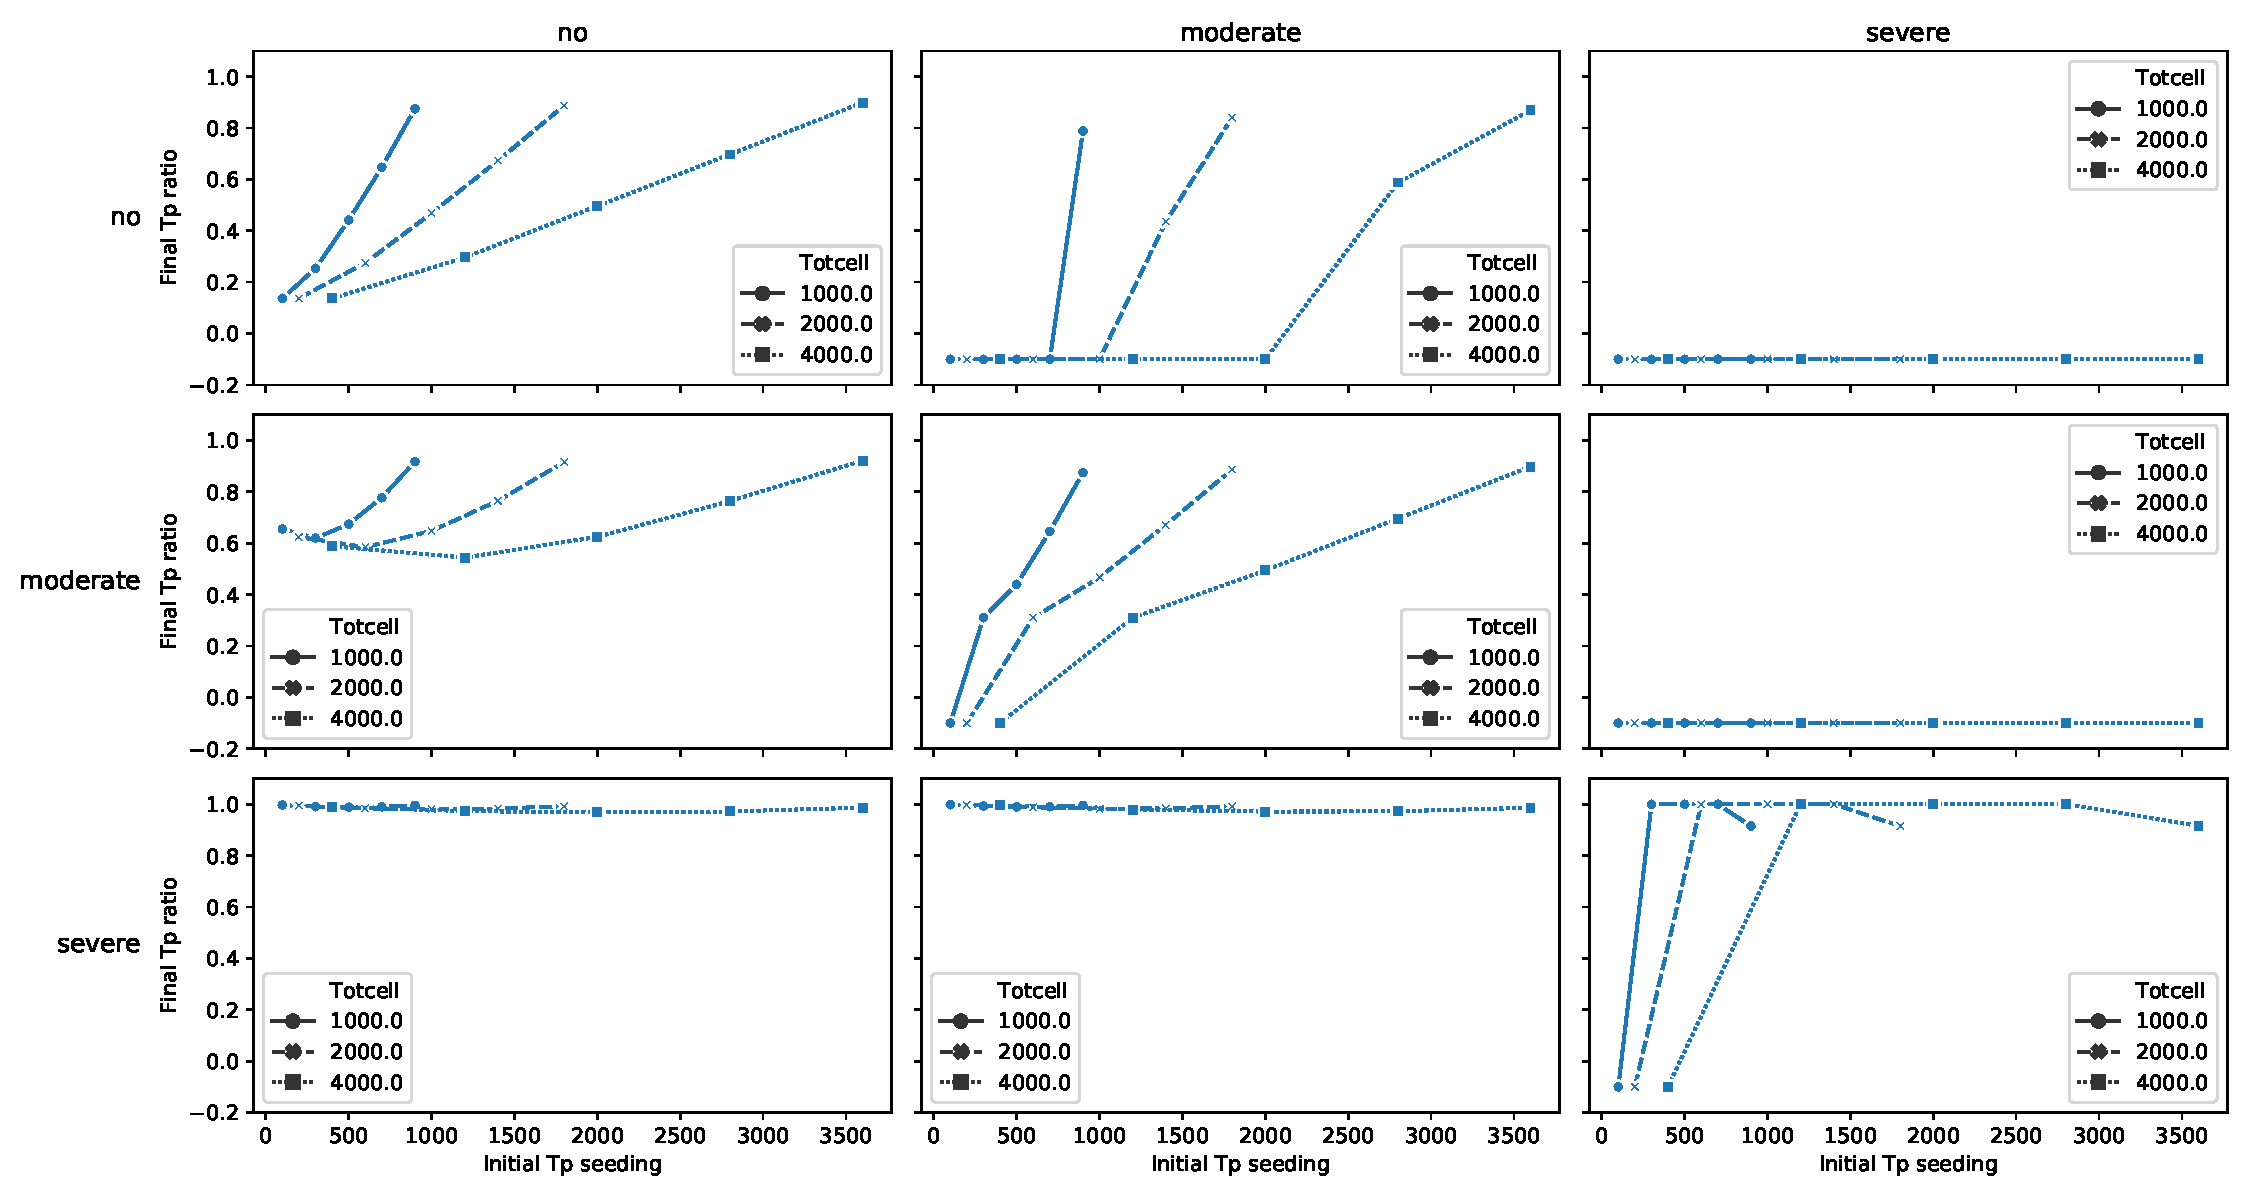
\includegraphics[width=\textwidth]{Tpos-Tpro_cases_test}
    \caption{$test$ limitations. Columns: $T^p\ test$ limitation, Rows: $T^+\ test$ limitation.}
    \label{fig_Tpos-Tpro_cases_test}
  \end{subfigure}
  \begin{subfigure}[b]{\textwidth}
    \centering
    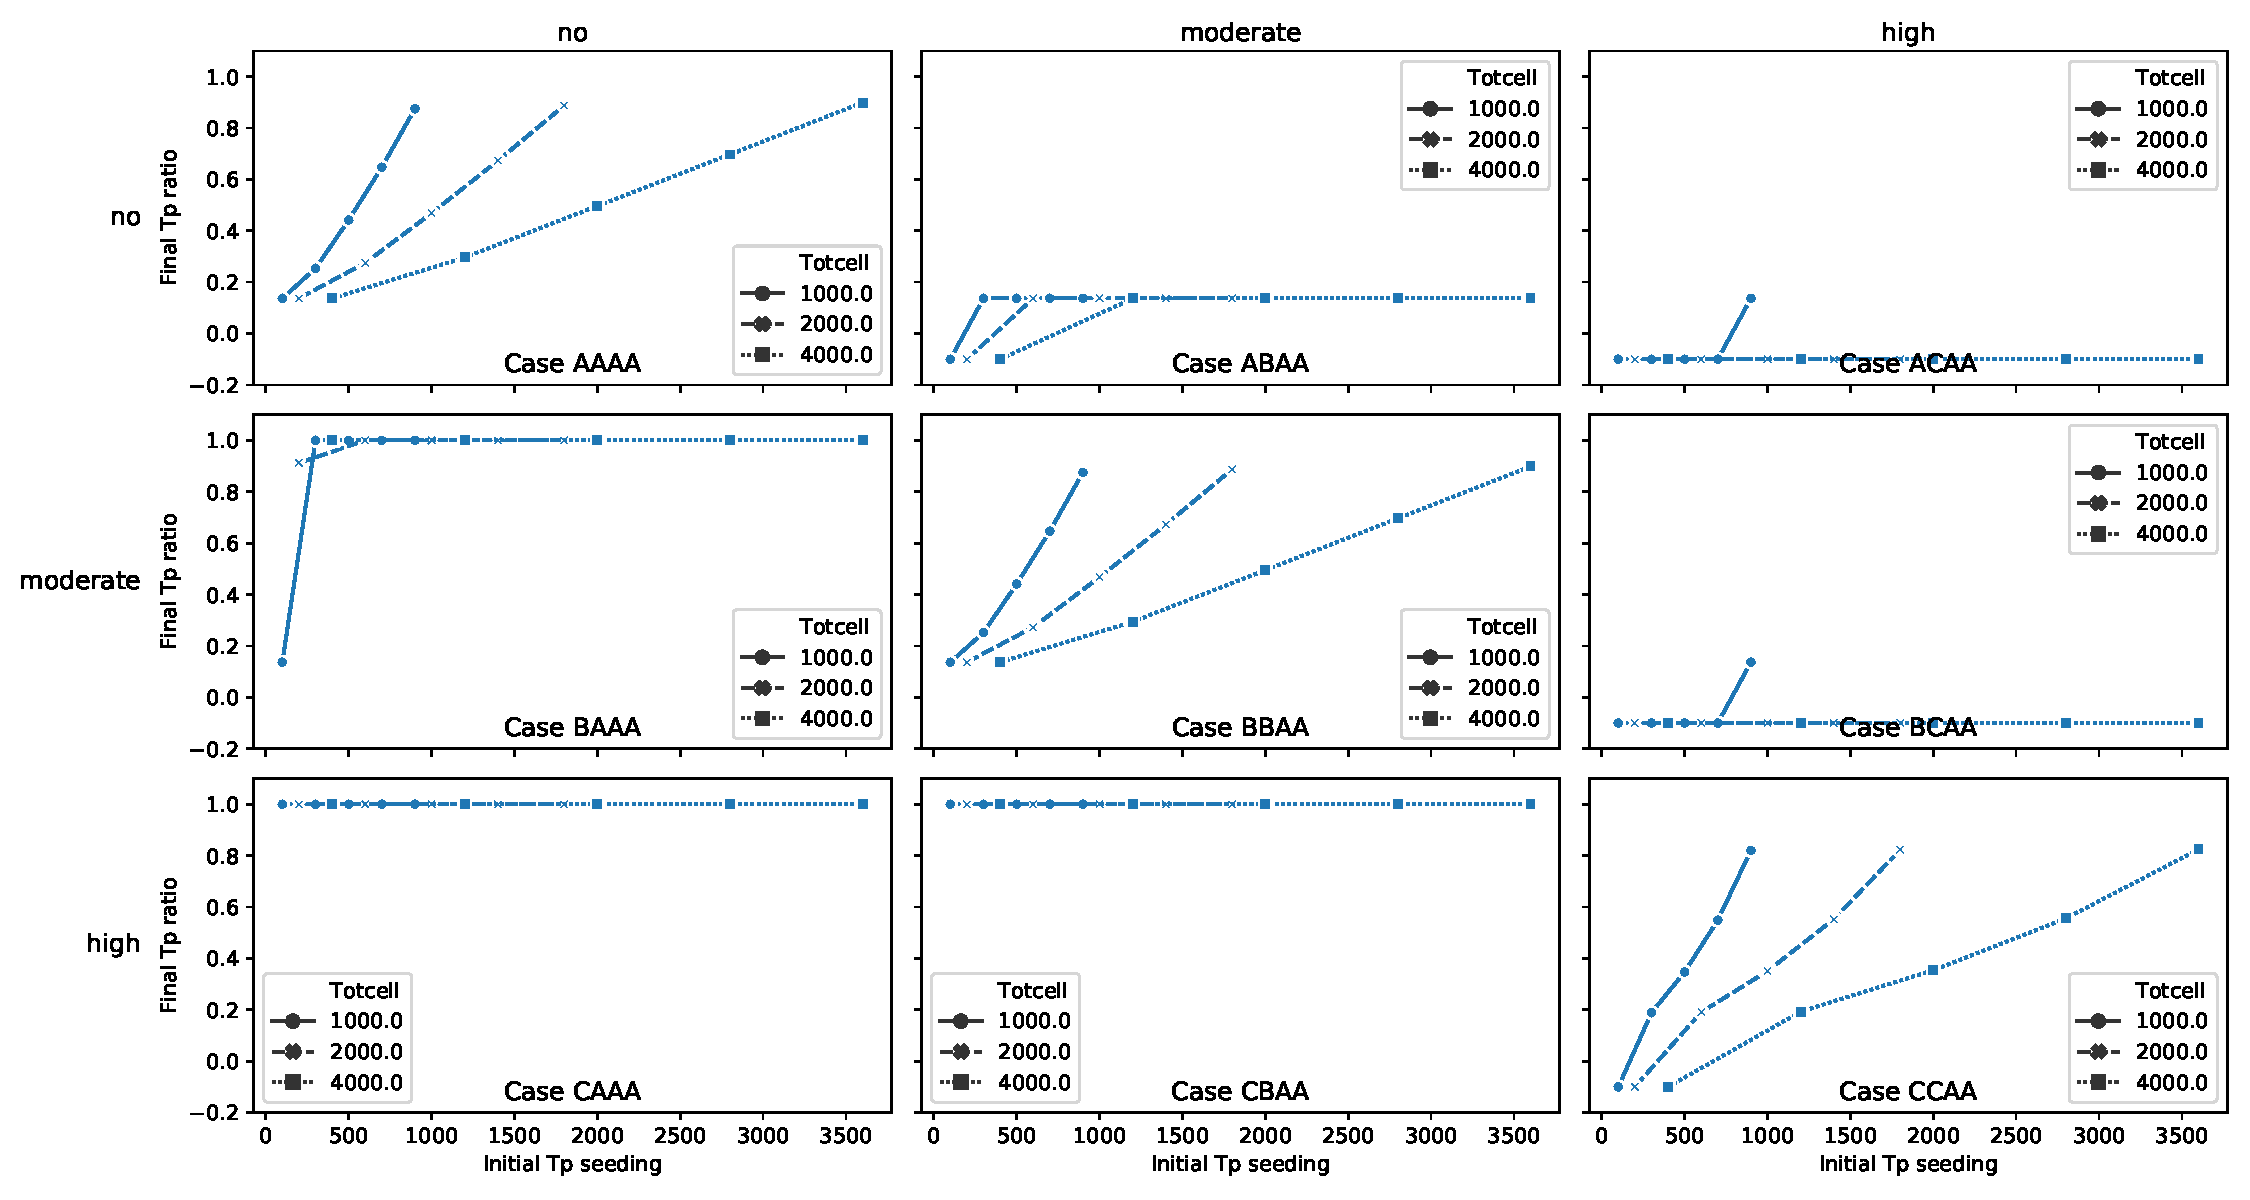
\includegraphics[width=\textwidth]{Tpos-Tpro_cases_o2}
    \caption{$O_2$ limitations. Columns: $T^p\ O_2$ limitation, Rows: $T^+\ O_2$ limitation.}
    \label{fig_Tpos-Tpro_cases_o2}
  \end{subfigure}
  \caption[Final $T^p$ ratio of pairwise $T^+ - T^p$ runs under different cases]{Final $T^p$ ratio of pairwise $T^+ - T^p$ runs under different cases. Note: Ratio = -0.1 is used when both cell types go extinct.}
\end{figure}
\begin{figure}[h!]\ContinuedFloat
  \begin{subfigure}[b]{\textwidth}
    \centering
    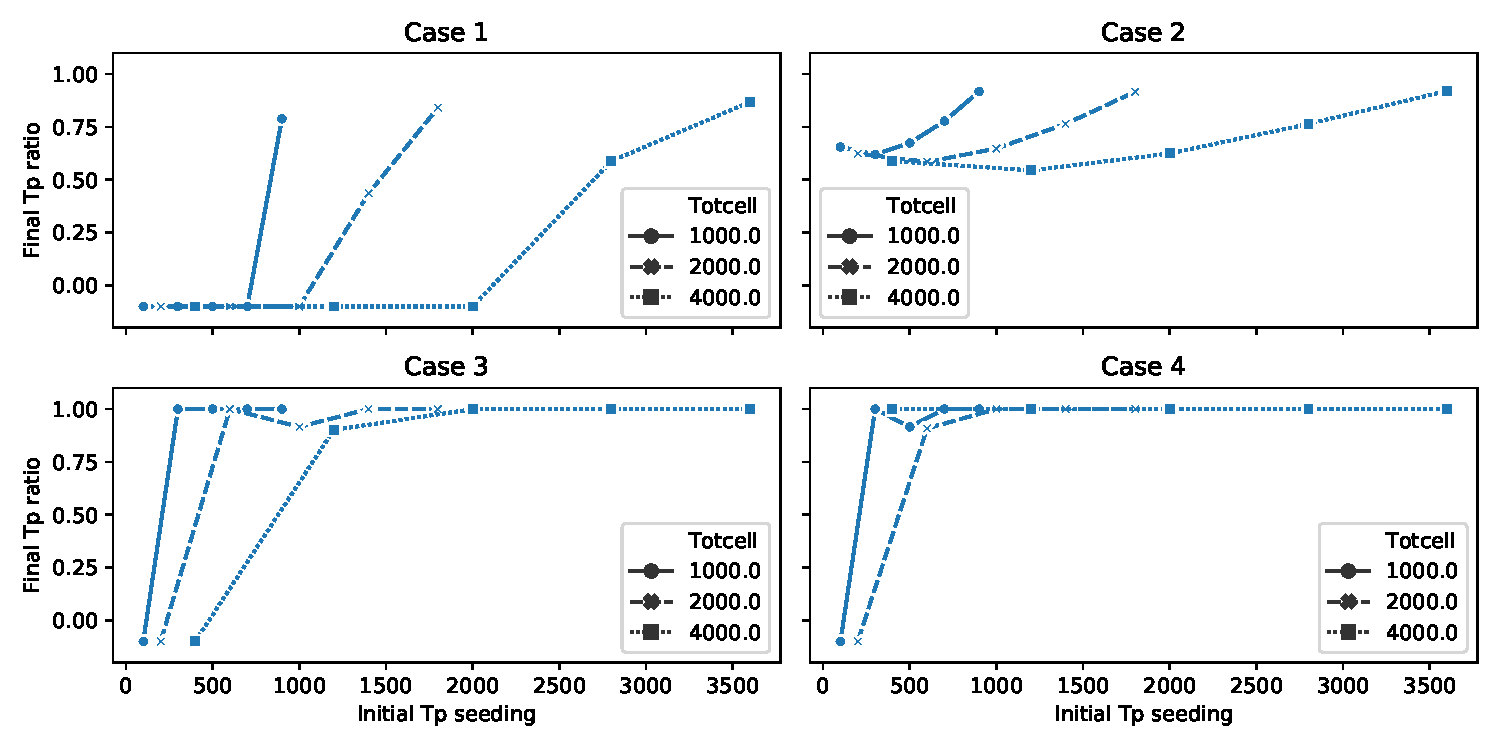
\includegraphics[width=\textwidth]{Tpos-Tpro_cases}
    \caption{Combination  of $test$ and $O_2$ limitations. Columns: $T^+,T^p\ test$ limitations, Rows: Columns: $T^+,T^p\ O_2$ limitations.}
    \label{fig_Tpos-Tpro_cases_combi}
  \end{subfigure}
  \caption[]{Final $T^p$ ratio of pairwise $T^+ - T^p$ runs under different cases. Note: Ratio = -0.1 is used when both cell types go extinct. (cont.)}
  \label{fig_Tpos-Tpro_cases}
\end{figure}

\newpage

\section{All 3 celltypes}
\subsection{Efficiency}
To simplify things, the resource limitations as described in the previous sections can instead be considered as efficiencies of the cell types in utilization of a particular resource. A cell with a high efficiency for a resource would be limited less by that resource whereas a cell with low efficiency for a resource would be severely limited by that resource.

With all three cell types, the number of combinations and permutations increase combinatorially, and sifting through such a massive pile of data is a daunting prospect. So, we are starting with a simpler case of the same strategy for all three cell types. The different efficiency levels and their corresponding values for lower and upper limits are given in \autoref{tab_efficiencies}.

\begin{longtable}[c]{|l|l|l|l|}
  \hline  \multicolumn{1}{|c|}{\textbf{Resource}} & \multicolumn{1}{c|}{\textbf{Efficiency}} & \multicolumn{1}{c|}{\textbf{lower limit}} & \multicolumn{1}{c|}{\textbf{upper limit}}  \\ \hline
  \endhead

  \hline \multicolumn{4}{|r|}{{Continued on next page}} \\ \hline
  \endfoot

  \endlastfoot

  \multirow{3}{*}{Oxygen} & Low Efficiency & 0.4 & 1.0 \\ \cline{2-4}
  & Null Efficiency & 0.0 & 1.0 \\ \cline{2-4}
  & High Efficiency & 0.0 & 0.1 \\ \hline
  \multirow{3}{*}{Testosterone} & Low Efficiency & 0 & 0.3 \\ \cline{2-4}
  & High Efficiency & 0 & 0.1 \\ \hline

  \caption{Table of limits corresponding to efficiencies for different resources}
  \label{tab_efficiencies}
\end{longtable}

The following were observed from the different cases as visualised is \autoref{fig_all3}
\begin{enumerate}
  \item Barring the case with high efficiencies for both testosterone and oxygen, $T^p$ and $T^+$ goes extinct for the lowest equal seeding densities regardless with the total amounting to 1000.
  \item With low testosterone efficiency, $T^p$ and $T^+$ go extinct at all the equal seeding densities regardless of their oxygen efficiencies. $T^-$ isn't affected by the testosterone limitation and can outcompete the other cells. However, when $T^p$ is seeded at 8 times the density of the other cell types, co-existence is achieved.
  \item $T^-$ seems to have an advantage when the oxygen efficiencies are lower. While this difference can be seen clearly with the reduction in final $T^-$ ratio from low to null oxygen efficiency, the difference between null and high oxygen efficiency is minor.
\end{enumerate}

\begin{figure}[h!]
\centering
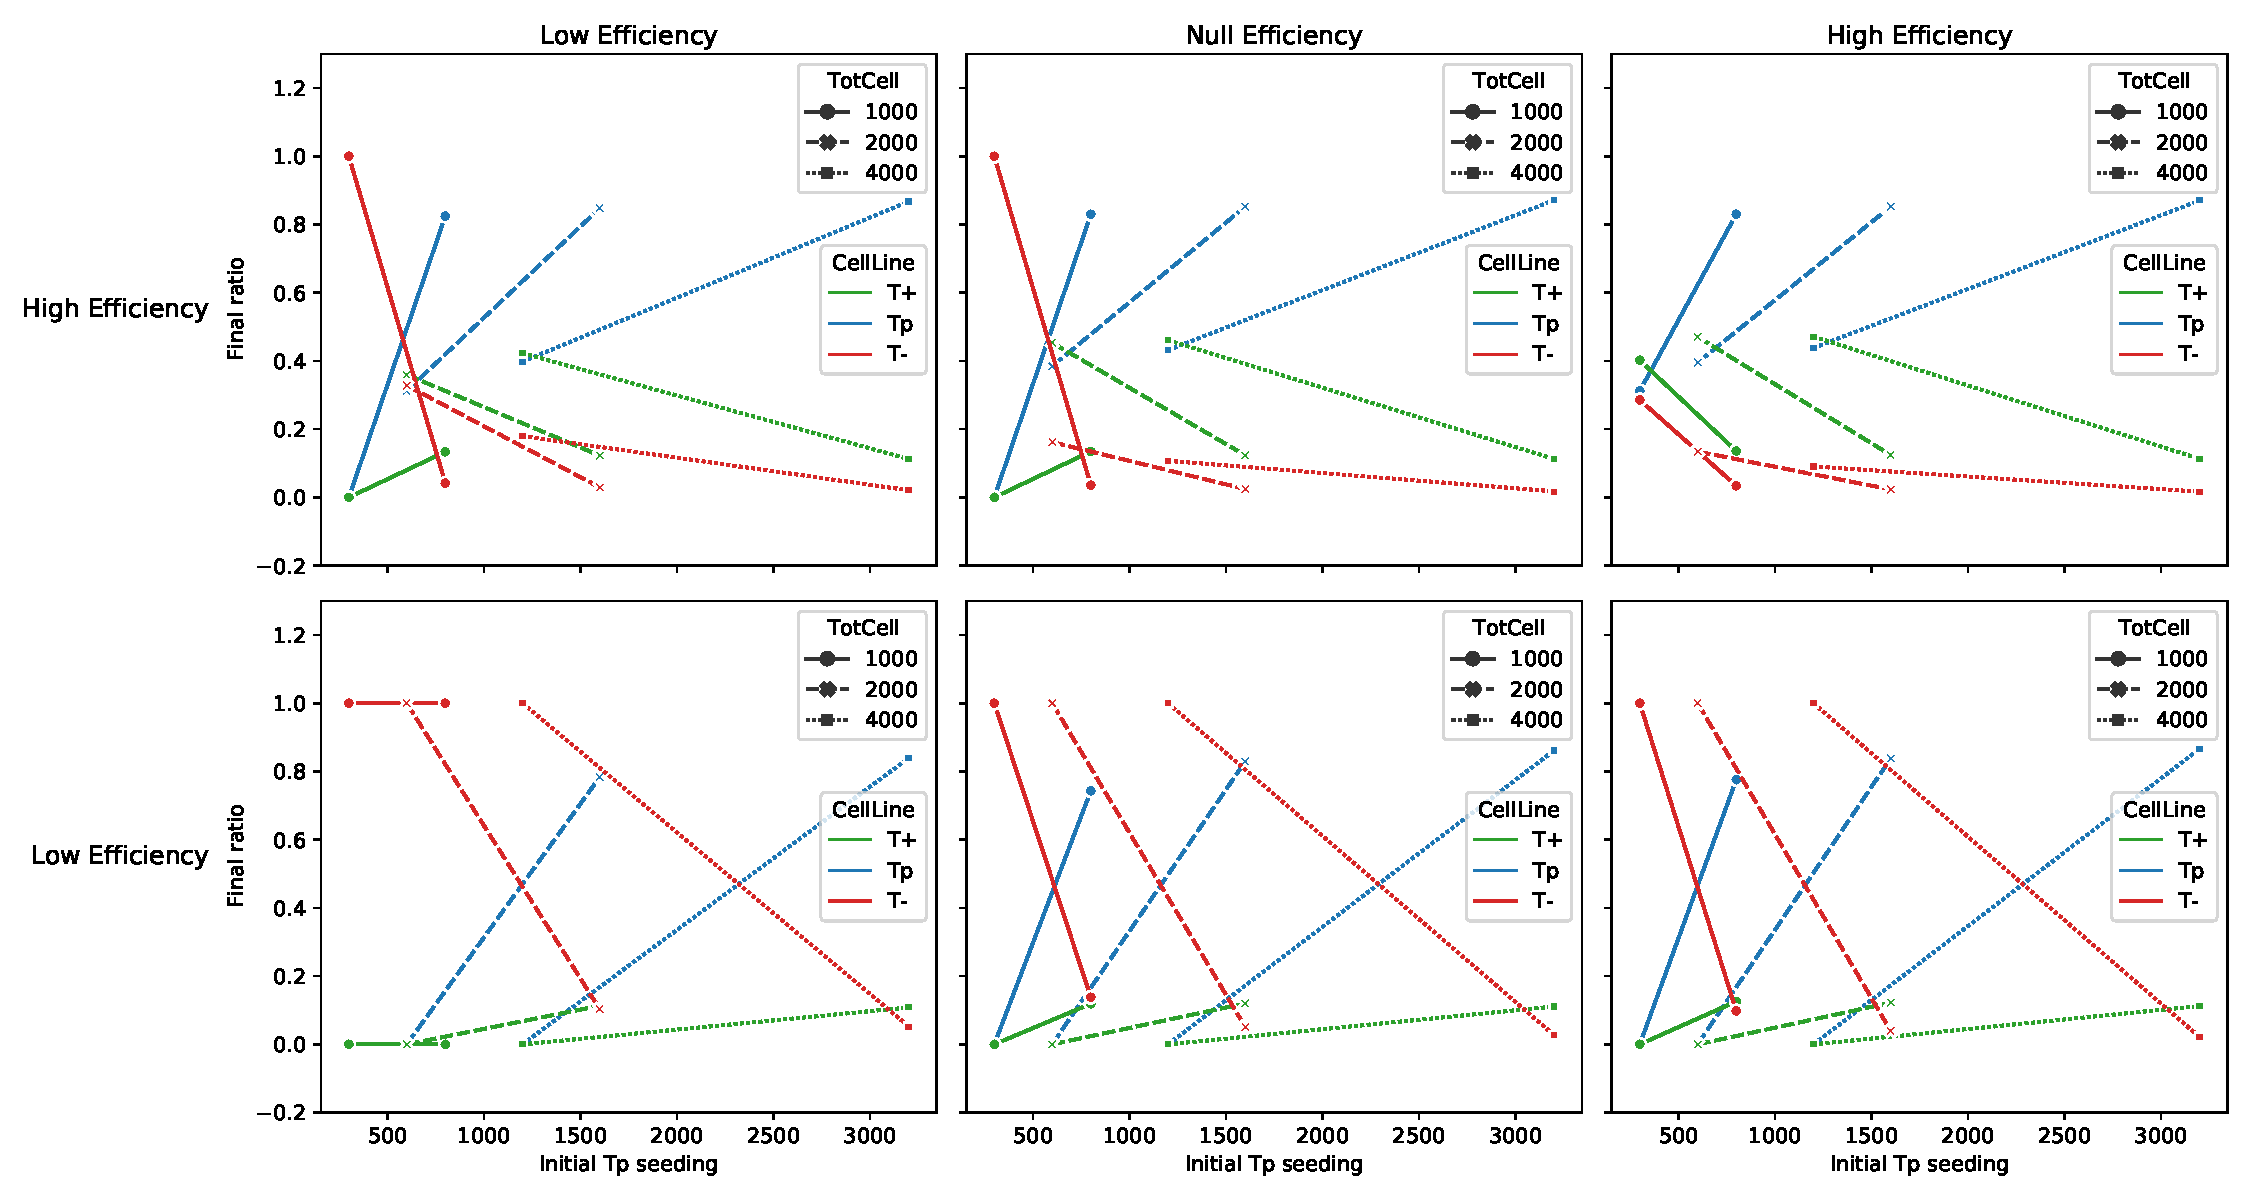
\includegraphics[width=\textwidth]{All3_efficiency}
\caption[Final ratio of all 3 cell type runs under different efficiencies]{Final ratio of all 3 cell type runs under different oxygen efficiency (columns) and testosterone efficiency (rows).}
\label{fig_all3}
\end{figure}
